\documentclass{article}

\def\ParSkip{} 
% Packages
\usepackage{amssymb,amsmath,amsthm,bbm}
\usepackage{verbatim,float,url,dsfont}
\usepackage{graphicx,subfigure,psfrag}
\usepackage{algorithm,algorithmic}
\usepackage{mathtools,enumitem}
\usepackage{multirow}
\usepackage{ragged2e}
\usepackage{xr-hyper}
\usepackage{array}

\usepackage[colorlinks=true,citecolor=blue,urlcolor=blue,linkcolor=blue]{hyperref}
\usepackage[margin=1in]{geometry}
\usepackage[round]{natbib}

\usepackage[utf8]{inputenc} % allow utf-8 input
\usepackage[T1]{fontenc}    % use 8-bit T1 fonts
\usepackage{booktabs}       % professional-quality tables
\usepackage{nicefrac}         % compact symbols for 1/2, etc.
\usepackage{microtype}      % microtypography

\ifdefined\TimesFont 
\usepackage{times} % use times font
\fi

\ifdefined\ParSkip 
\usepackage{parskip} % use par skip
\fi

% Theorems and such
\newtheorem{theorem}{Theorem}
\newtheorem{lemma}{Lemma}
\newtheorem{corollary}{Corollary}
\newtheorem{proposition}{Proposition}
\theoremstyle{definition}
\newtheorem{remark}{Remark}
\newtheorem{definition}{Definition}

% Assumption
\newtheorem*{assumption*}{\assumptionnumber}
\providecommand{\assumptionnumber}{}
\makeatletter
\newenvironment{assumption}[2]{
  \renewcommand{\assumptionnumber}{Assumption #1#2}
  \begin{assumption*}
  \protected@edef\@currentlabel{#1#2}}
{\end{assumption*}}
\makeatother

% Widebar
\makeatletter
\newcommand*\rel@kern[1]{\kern#1\dimexpr\macc@kerna}
\newcommand*\widebar[1]{%
  \begingroup
  \def\mathaccent##1##2{%
    \rel@kern{0.8}%
    \overline{\rel@kern{-0.8}\macc@nucleus\rel@kern{0.2}}%
    \rel@kern{-0.2}%
  }%
  \macc@depth\@ne
  \let\math@bgroup\@empty \let\math@egroup\macc@set@skewchar
  \mathsurround\z@ \frozen@everymath{\mathgroup\macc@group\relax}%
  \macc@set@skewchar\relax
  \let\mathaccentV\macc@nested@a
  \macc@nested@a\relax111{#1}%
  \endgroup
}
\makeatother

% Min and max 
\DeclareMathOperator*{\argmin}{argmin}
\DeclareMathOperator*{\argmax}{argmax}
\DeclareMathOperator*{\minimize}{minimize}
\DeclareMathOperator*{\maximize}{maximize}
\DeclareMathOperator*{\find}{find}
\DeclareMathOperator{\st}{subject\,\,to}

% Other operators
\DeclareMathOperator{\Cov}{Cov}
\DeclareMathOperator{\Var}{Var}
\DeclareMathOperator{\dm}{dim}
\DeclareMathOperator{\col}{col}
\DeclareMathOperator{\row}{row}
\DeclareMathOperator{\nul}{null}
\DeclareMathOperator{\rank}{rank}
\DeclareMathOperator{\nuli}{nullity}
\DeclareMathOperator{\spa}{span}
\DeclareMathOperator{\sign}{sign}
\DeclareMathOperator{\supp}{supp}
\DeclareMathOperator{\diag}{diag}
\DeclareMathOperator{\aff}{aff}
\DeclareMathOperator{\conv}{conv}
\DeclareMathOperator{\dom}{dom}
\DeclareMathOperator{\tr}{tr}
\DeclareMathOperator{\df}{df}

% Other shortcuts 
\def\R{\mathbb{R}}
\def\C{\mathbb{C}}
\def\E{\mathbb{E}}
\def\P{\mathbb{P}}
\def\T{\mathsf{T}}
\def\half{\frac{1}{2}}
\def\df{\mathrm{df}}
\def\hy{\hat{y}}
\def\hf{\hat{f}}
\def\hmu{\hat{\mu}}
\def\halpha{\hat{\alpha}}
\def\hbeta{\hat{\beta}}
\def\htheta{\hat{\theta}}
\def\indep{\perp\!\!\!\perp}
\def\th{^{\textnormal{th}}}

\def\cA{\mathcal{A}}
\def\cB{\mathcal{B}}
\def\cD{\mathcal{D}}
\def\cE{\mathcal{E}}
\def\cF{\mathcal{F}}
\def\cG{\mathcal{G}}
\def\cK{\mathcal{K}}
\def\cH{\mathcal{H}}
\def\cI{\mathcal{I}}
\def\cL{\mathcal{L}}
\def\cM{\mathcal{M}}
\def\cN{\mathcal{N}}
\def\cP{\mathcal{P}}
\def\cS{\mathcal{S}}
\def\cT{\mathcal{T}}
\def\cW{\mathcal{W}}
\def\cX{\mathcal{X}}
\def\cY{\mathcal{Y}}
\def\cZ{\mathcal{Z}}


\title{Lecture 7: Exponential Smoothing with Trend and Seasonality \\ 
\Large And a Brief Tour of Other Popular Forecasting Methods \\ \smallskip
\large Introduction to Time Series, Fall 2023 \\ \smallskip
Ryan Tibshirani}
\date{}

\begin{document}
\maketitle
\RaggedRight
\vspace{-50pt}

Related reading: Chapters 8, 9.10, 12.2, and 12.4 of Hyndman and Athanasopoulos
(HA).

\section{Simple exponential smoothing}

\begin{itemize}
\item Exponential smoothing is arguably the other---outside of ARIMA---most 
  popular basic framework for forecasting in time series. These two frameworks
  bear a neat connection, which you saw at the end of the last lecture on ARIMA,
  and which we'll revisit a bit later in this lecture

\item We'll begin with the simplest possible exponential smoother, called
  (unsurprisingly?) \emph{simple exponential smoothing} (SES). This constructs 
  a 1-step ahead forecast via
  \begin{equation}
  \label{eq:ses}
  \hat{x}_{t+1 | t }= \alpha x_t + (1-\alpha) \hat{x}_{t | t-1}
  \end{equation}
  where $\alpha \in [0,1]$ is a parameter to be estimated

\item In other words, the SES forecast \eqref{eq:ses} is a weighted combination 
  of the current observation $x_t$ and the previous forecast \smash{$\hat{x}_{t
      | t-1}$} 

\item By unraveling the iteration, which is basically the same calculation that
  we did in the ARIMA lecture (but now in the opposite direction), this can also
  be written as    
  \begin{equation}
  \label{eq:ses-exp}
  \hat{x}_{t+1 | t} = \alpha x_t + \alpha (1-\alpha) x_{t-1} + \alpha
  (1-\alpha)^2 x_{t-2} + \dots
  \end{equation}
  This explains its name, since observations $x_{t-k}$ that are $k$ steps into 
  the past are exponentially-downweighted, with weight $(1-\alpha)^k$  

\item  (Note: we are being intentionally vague here about the boundary 
  condition. In ARIMA, to develop the theory cleanly, we let time extend back to
  $-\infty$. In  exponential smoothing, we instead usually index time starting
  at $t = 0$, in which case the right-hand side in \eqref{eq:ses-exp} would end
  with $\alpha (1-\alpha)^t x_0$, and we often take $x_0 = 0$ for simplicity)

\item To make $h$-step ahead forecasts, we iterate \eqref{eq:ses}, where (as 
  usual) we replace future observations by their forecasts. This simply  
  yields \smash{$\hat{x}_{t+2 | t} = \alpha \hat{x}_{t+1 | t} + (1-\alpha)
    \hat{x}_{t+1 | t} = \hat{x}_{t+1 | t}$}, and in general, 
  \begin{equation}
  \label{eq:ses-h}
  \hat{x}_{t+h | t} = \alpha x_t + (1-\alpha) \hat{x}_{t | t-1}
  \end{equation}
  for all horizons $h \geq 1$. That is, SES generates \emph{flat} forecast
  trajectories. We'll see how to extend this to accomodate a trend, shortly  

\item While SES smoothing is already very intuitive, we can motivate it in
  different way, as follows. The \emph{naive flatline forecaster} produces
  forecasts via
  \begin{equation}
  \label{eq:flatline-h}
  \hat{x}_{t+h | t} = x_t 
  \end{equation}
  i.e., it just propogates the last observation forward. Meanwhile, the
  \emph{naive average forecaster} produces forecasts via
  \begin{equation}
  \label{eq:average-h}
  \hat{x}_{t+h | t} = \frac{1}{t} \sum_{i=1}^t x_i
  \end{equation}
  Often we want something in between these two extremes, and that something is  
  given to us by exponential smoothing, recalling the form in \eqref{eq:ses-exp} 
\end{itemize}

\subsection{Component form}

\begin{itemize}
\item For the developments that follow, it is helpful to rewrite the SES forecast
  \eqref{eq:ses-h} in what is known as \emph{component form}

\item Specifically, we think of a ``hidden'' level $\ell_t$ that we are tracking
  over time, that base our forecasts on:
  \begin{equation}
  \label{eq:ses-component}
  \begin{aligned}
  \hat{x}_{t+h | t} &= \ell_t \\
  \ell_t &= \alpha x_t + (1-\alpha) \ell_{t-1}
  \end{aligned}
  \end{equation}

\item The representation in \eqref{eq:ses-component} may appear as kind of a
  trivial rewriting of \eqref{eq:ses-h}, where we replace \smash{$\hat{x}_{t+1 |
      t}$} by $\ell_t$, and \smash{$\hat{x}_{t | t-1}$} by $\ell_{t-1}$. 
  Nonetheless, it serve as a useful jumping off point to extend the model in the 
  next section   

\item Before moving on, we give a brief example of SES from HA, to forecast
  internet useage per minute. The data and SES forecast are shown in Figure
  \ref{fig:internet}, top row. In order to carry out the forecast, we have to
  estimate the smoothing parameter $\alpha$ in \eqref{eq:ses-component}. This is 
  typically done by maximum likelihood (more later), and is what is implemented
  as the default in the \verb|ETS()| function in the \verb|fable| package 

\begin{figure}[p]
\centering
%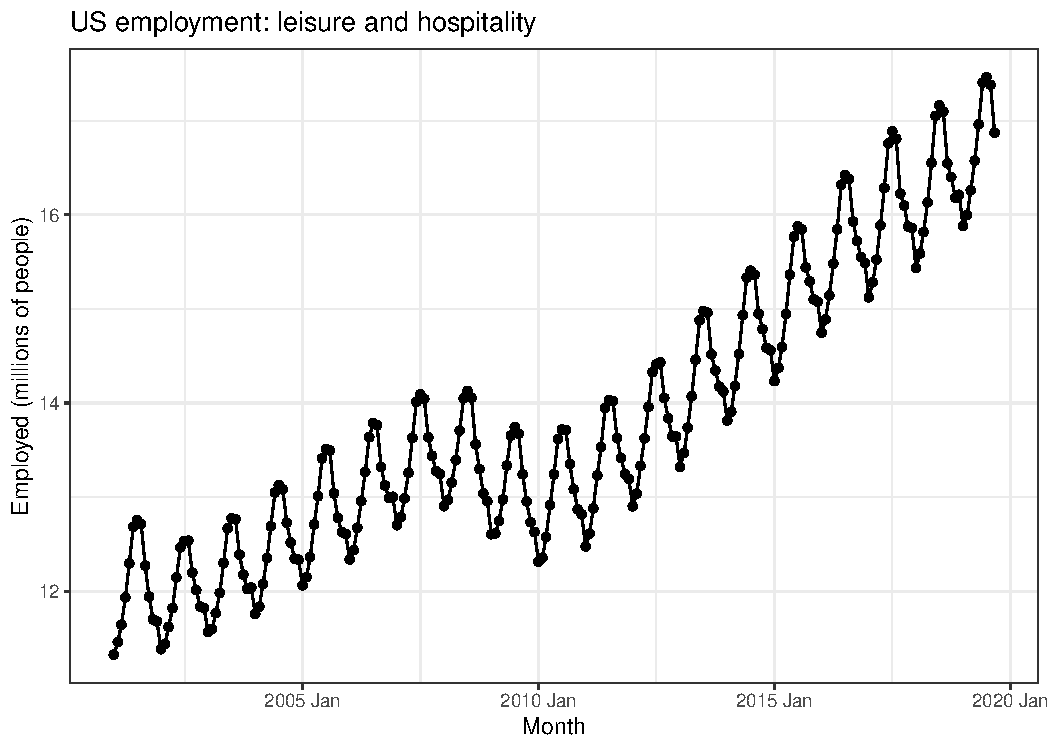
\includegraphics[width=0.6\textwidth]{fig/leisure-1.pdf}
%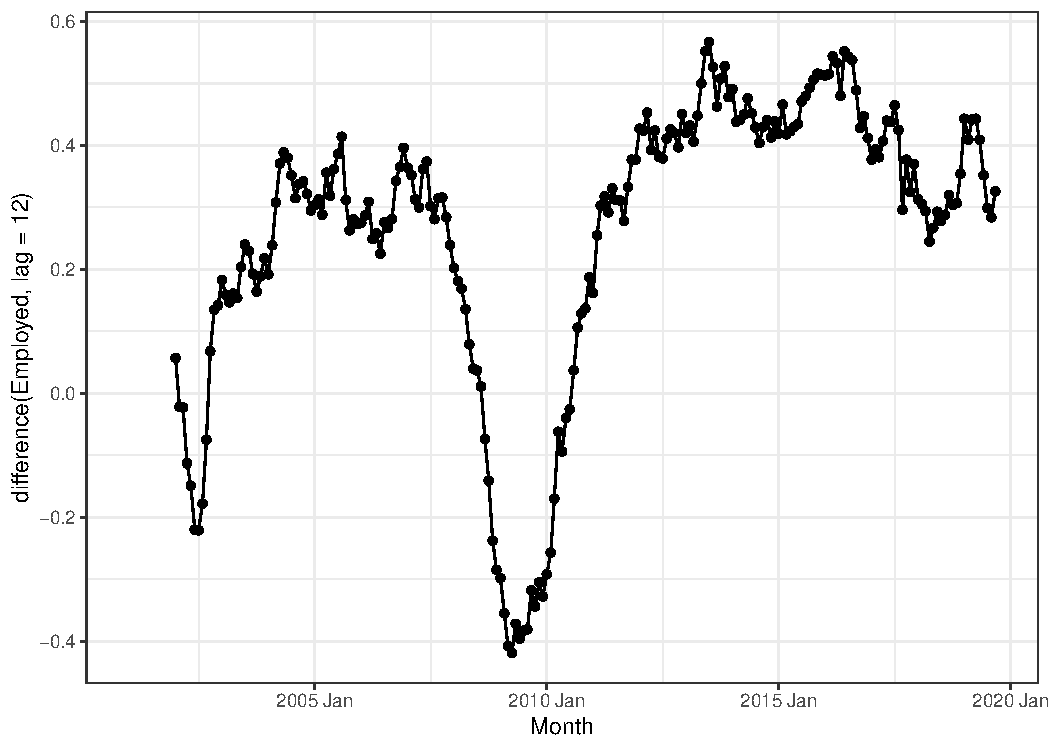
\includegraphics[width=0.6\textwidth]{fig/leisure-2.pdf}
%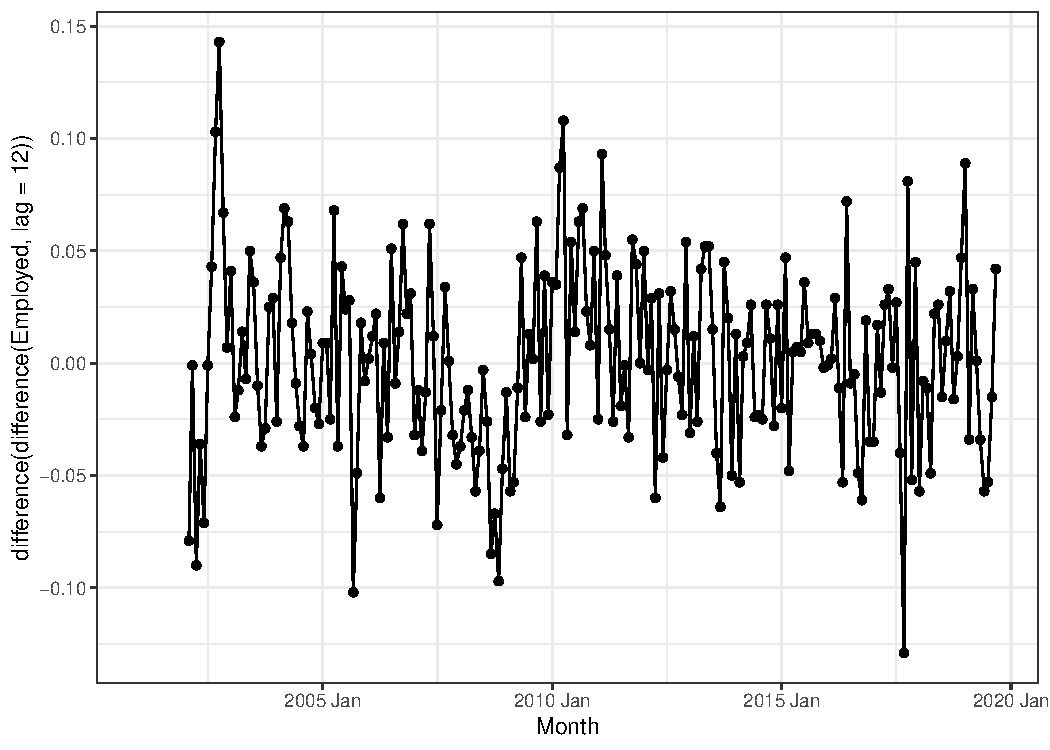
\includegraphics[width=0.6\textwidth]{fig/leisure-3.pdf}
\caption{ } 
\label{fig:internet}
\end{figure}

\item The forecast from SES is not very impressive, and honestly, in general,
  SES should probably only be viewed as a small step up from the naive
  forecasters \eqref{eq:flatline-h}, \eqref{eq:average-h} 

\item The forecast trajectory from SES is flat, by construction (as previously
  noted). Next we'll see how to extend the method to accommodate a linear trend  
\end{itemize}

\section{Trend extensions}

\begin{itemize}
\item Holt's linear trend
\end{itemize}

\subsection{Damped trends}

\begin{itemize}
\item 
\end{itemize}

\section{Seasonality extensions}

\begin{itemize}
\item Holt-Winters
\item dampening is also possible
\end{itemize}

\subsection{Multiplicative version}

\begin{itemize}
\item 
\item dampening is also possible
\end{itemize}

\section{ETS models}

\begin{itemize}
\item Multiplicative errors and trends
\item HA do not recommend multiplicative trend?
\end{itemize}

\subsection{State space representation}

\begin{itemize}
\item 
\end{itemize}

\subsection{Estimation and selection}

\begin{itemize}
\item 
\end{itemize}

\subsection{Forecasting}

\begin{itemize}
\item 
\end{itemize}

\subsection{ARIMA versus ETS}
\begin{itemize}
\item 
\end{itemize}

\section{Theta model}

\section{Prophet model}

\section{Neural network AR}



\end{document}
